\chapter{Multi-sensor Data Fusion}
\label{ch:Sensor Fusion}

\section{Introduction}
Multi-sensor data fusion is a multilevel, multifaceted process dealing with the detection, association, correlation, estimation, and combination of data and information from multiple sources to achieve refined state and identity estimation, and complete and timely assessments of situations and threat as define in \cite{Edward}. The primary objective of sensor data fusion is to combine sensory data from multiple disparate sources such that the outcome is less uncertain than the individual sensory information. 

When the information from more than one sensor is identical, a multi-sensor data fusion reduces the overall uncertainty of information, and if the information is not similar then it combines all information to make complex decisions that can not be possible by the use of a single sensor. In such a case, each sensor becomes complementary to the other.

\section{Types of Multi-sensor Data Fusion}
Based on the functional level of information abstraction, the data fusion is divided into three types as follows. 1. Feature Level, 2. Position Level, and 3. Attribute Level.  

\subsection{Feature Level Fusion}
It is a fusion that performs directly on object features. The sensory system is responsible for on-board computation to detect features from the environment, therefore the overall computational load on the system is reduced. The correlated features further fuse to observe the trend of entity of interest for instance weather forecasting, organizational management, detect the fault in mechanical systems, and medical diagnosis.
 
\subsection{Position Level Fusion}
Position level fusion aims to perform fusion directly on the observation data of the sensor or estimation of states in time and space. It is the most common sensor fusion method that has been used in many applications. It takes information from homogeneous sources and performs fusion to increase certainty. This type of sensor fusion has to deal with big input spaces because raw information from more than one source creates huge information space. Thus, the overall performance of the framework slows down as the number of sources increases. If there is any malfunction in a sensor modality, then the whole system generates ambiguous output.

\subsection{Attribute Level Fusion}
It selects the hypothesis or attributes from a set of presumptions generated by individual decision nodes. It is a high-level extraction of information that already has been reprocessed through feature-level processing. Typically, this type of fusion is used in target classification and recognition tasks. The outcome of this framework is improved accuracy in decision-making. Based on the level of information abstraction, it is divided into three layers as follows: decision-making layer, feature layer, and data layer fusion. The common flow chart of target attributes identification is shown in Fig. \ref{attributefusion}.

\begin{figure}
    \centering
    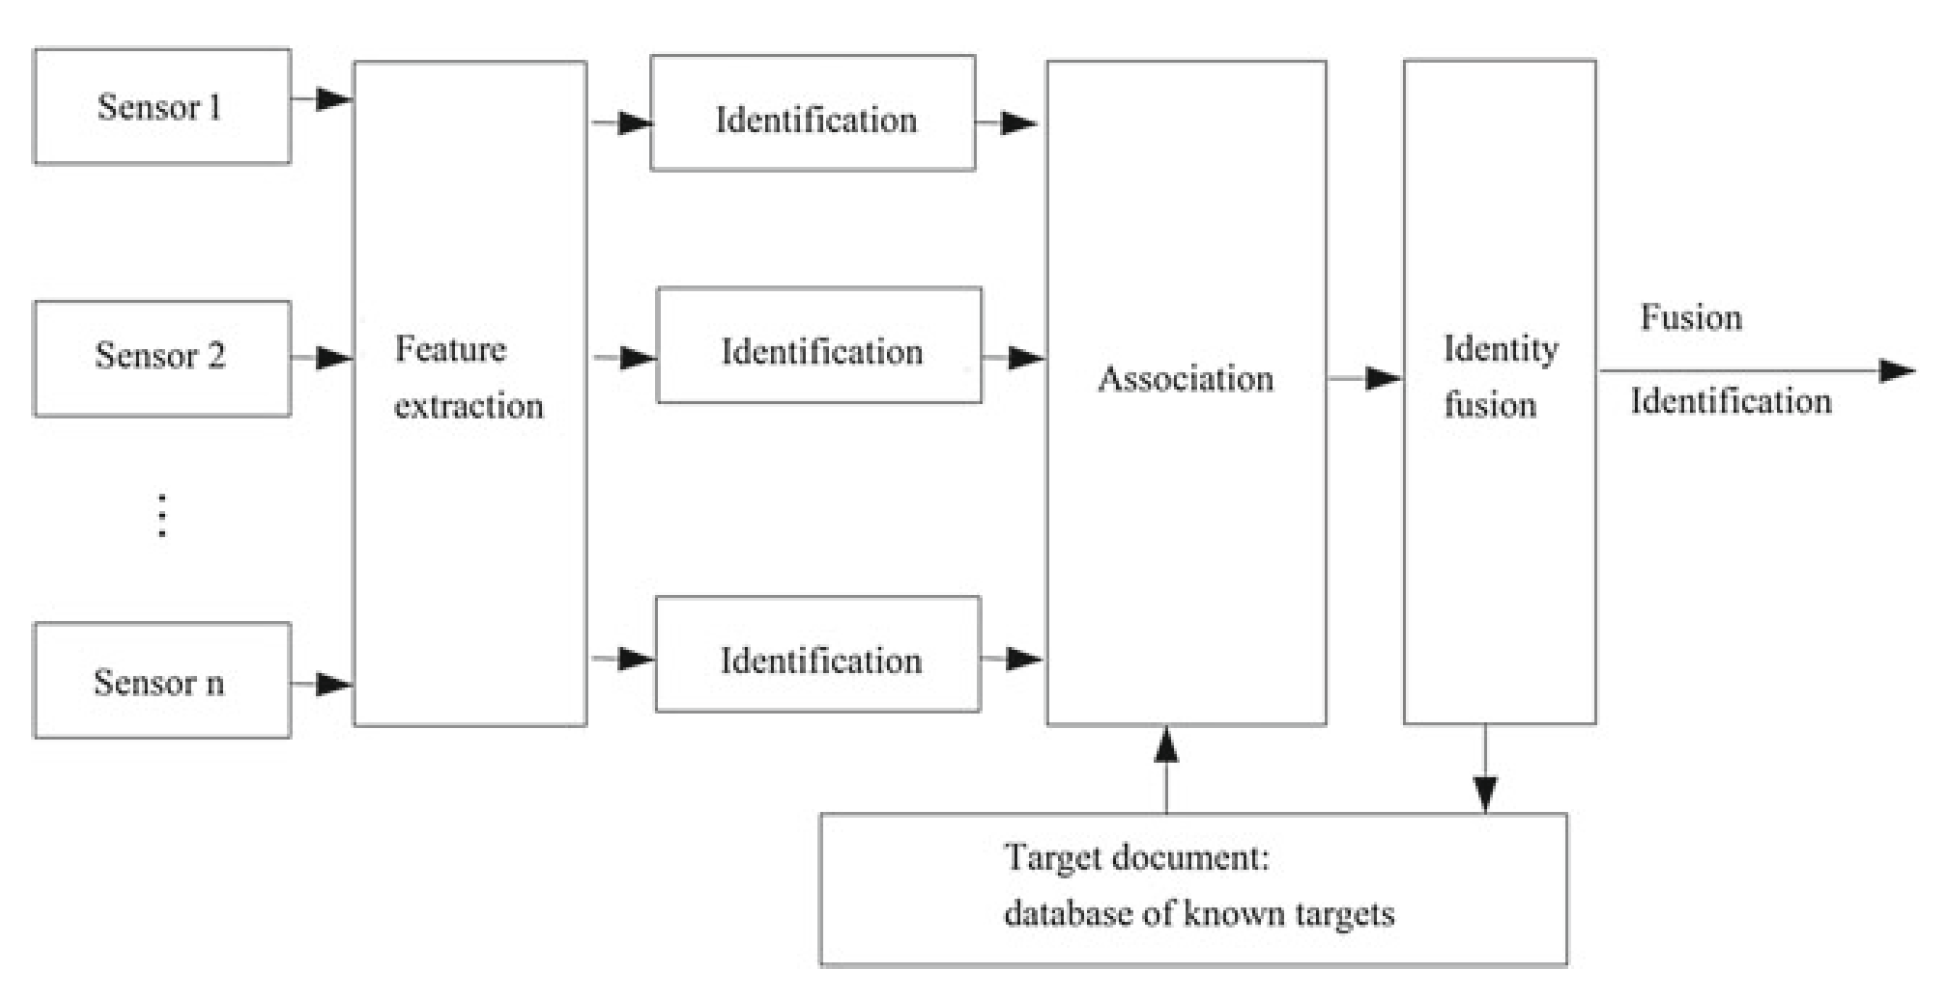
\includegraphics[width=0.7\textwidth]{Images/attributefusion.png}
    \caption{Attributes Identification Flow Chart \cite{yan}}
    \label{attributefusion}
\end{figure}

\section{Frameworks of Position Level Fusion}
In position level multi-sensor data fusion, there are three types of fusion architectures such as centralized, distributed, and compound or hybrid structure which are explained in the following subsections.

\subsection{Centralized Fusion Architecture}
In the centralized fusion structure, the raw data from the discrete sources are directly fed into the fusion framework. Firstly, the time fusion is performed on the time sequence of target observation and then multi-sensor spatial fusion is performed at the same time. It is used for object tracking and state estimation. The flow chart of the centralized fusion structure is shown in Fig. \ref{centralized}.  

\begin{figure}
    \centering
    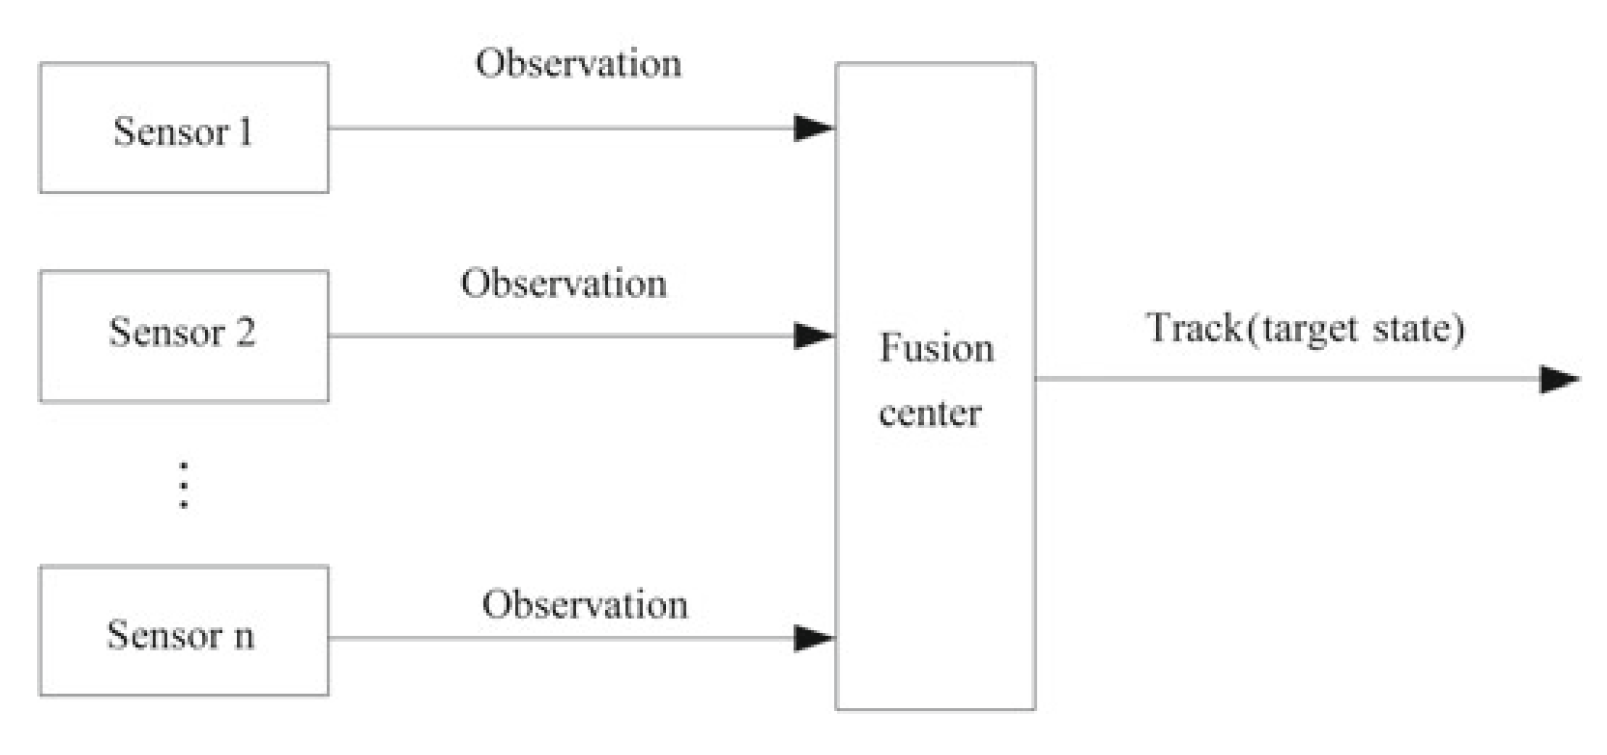
\includegraphics[width=0.9\textwidth]{Images/centralized.png}
    \caption{Centralized Fusion Architecture \cite{yan}}
    \label{centralized}
\end{figure}

\subsection{Distributed Fusion Architecture}
In the distributed tracking system, two levels of tracking are performed. Each sensor has its tracker to perform local level tracking, and all these tracking estimations fed into a global tracker or central level tracker to synthesizes the local estimation into a joint target estimation. The advantages of such type of architecture are it requires low communication bandwidth, fast computation speed, reliable and continuity. The schematic of distributed fusion structure is shown in Fig. \ref{distributed}. 

It is further divided into three types based on feedback from the central tracker such as distributed system without feedback, distributed system with feedback, and fully distributed. The first type is the most common type of architecture in which if any local tracker failure occurs it degrades the overall system performance. In the distributed system with feedback, the central node is fed back to each local node. The main advantage of such a structure is to detect failure or to supervise the local nodes. Furthermore, in the fully distributed structure, all the local nodes are connected with each other and the central node.   

\begin{figure}
    \centering
    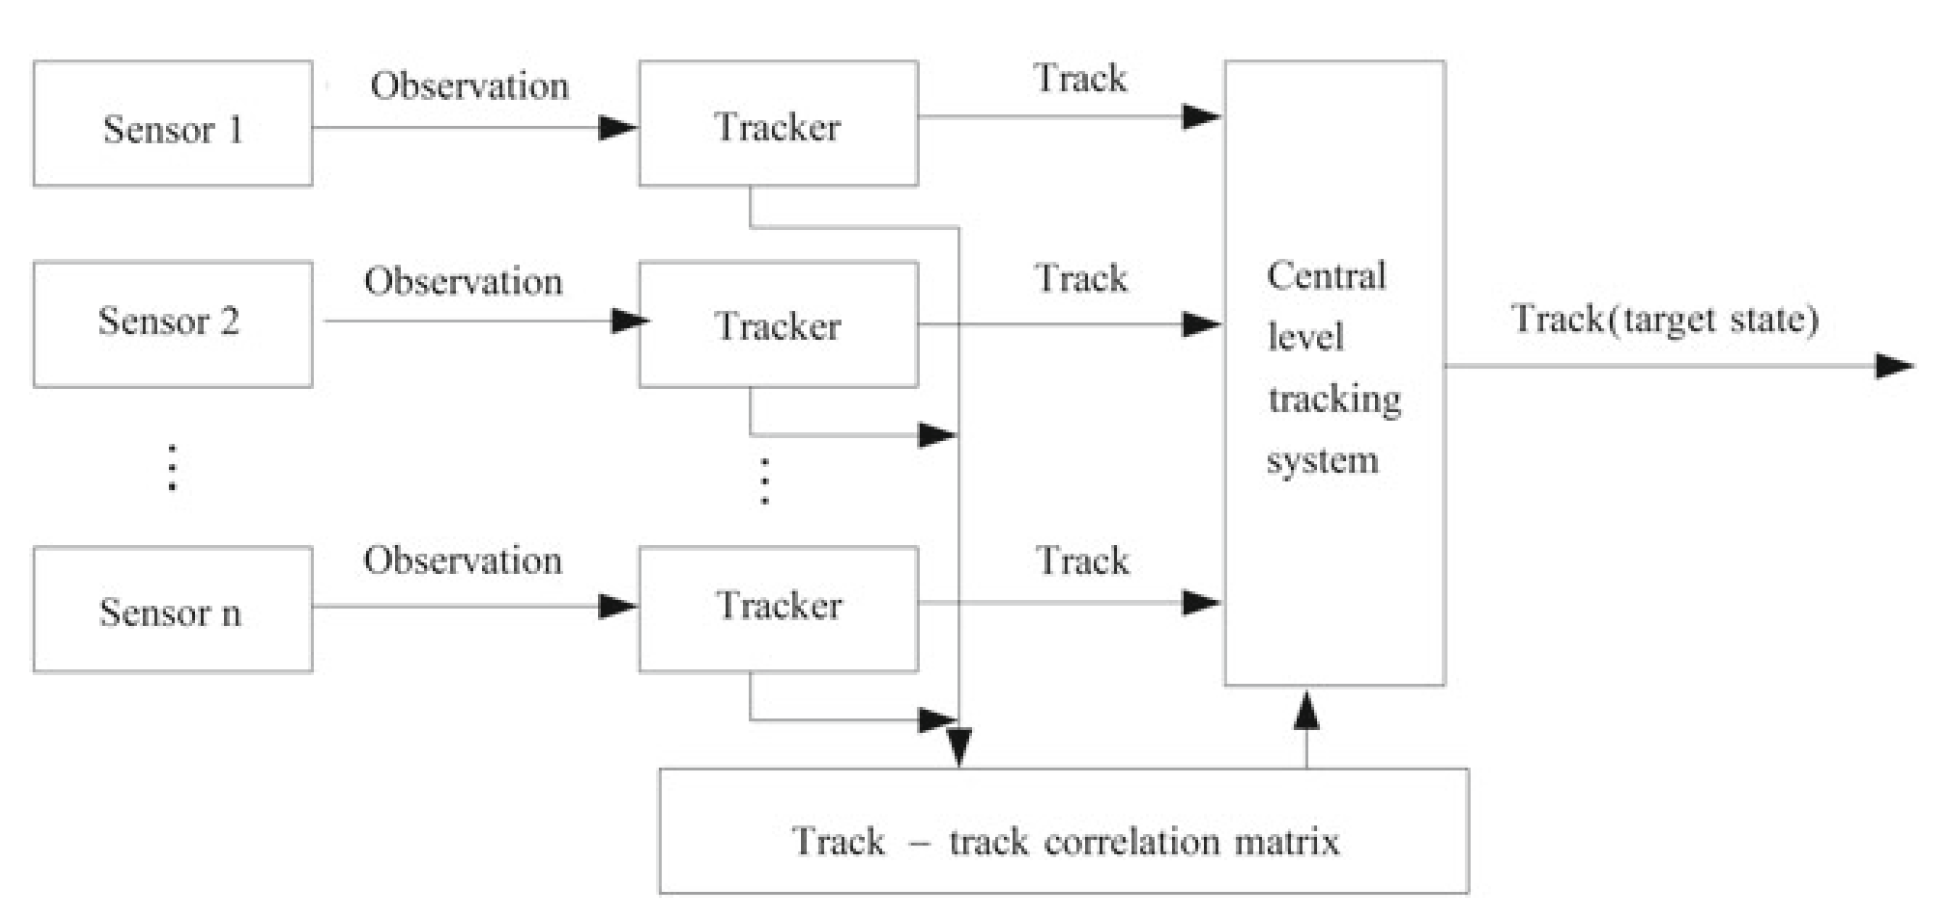
\includegraphics[width=0.9\textwidth]{Images/distributed.png}
    \caption{Distributed Fusion Architecture \cite{yan}}
    \label{distributed}
\end{figure}

\begin{figure}
    \centering
    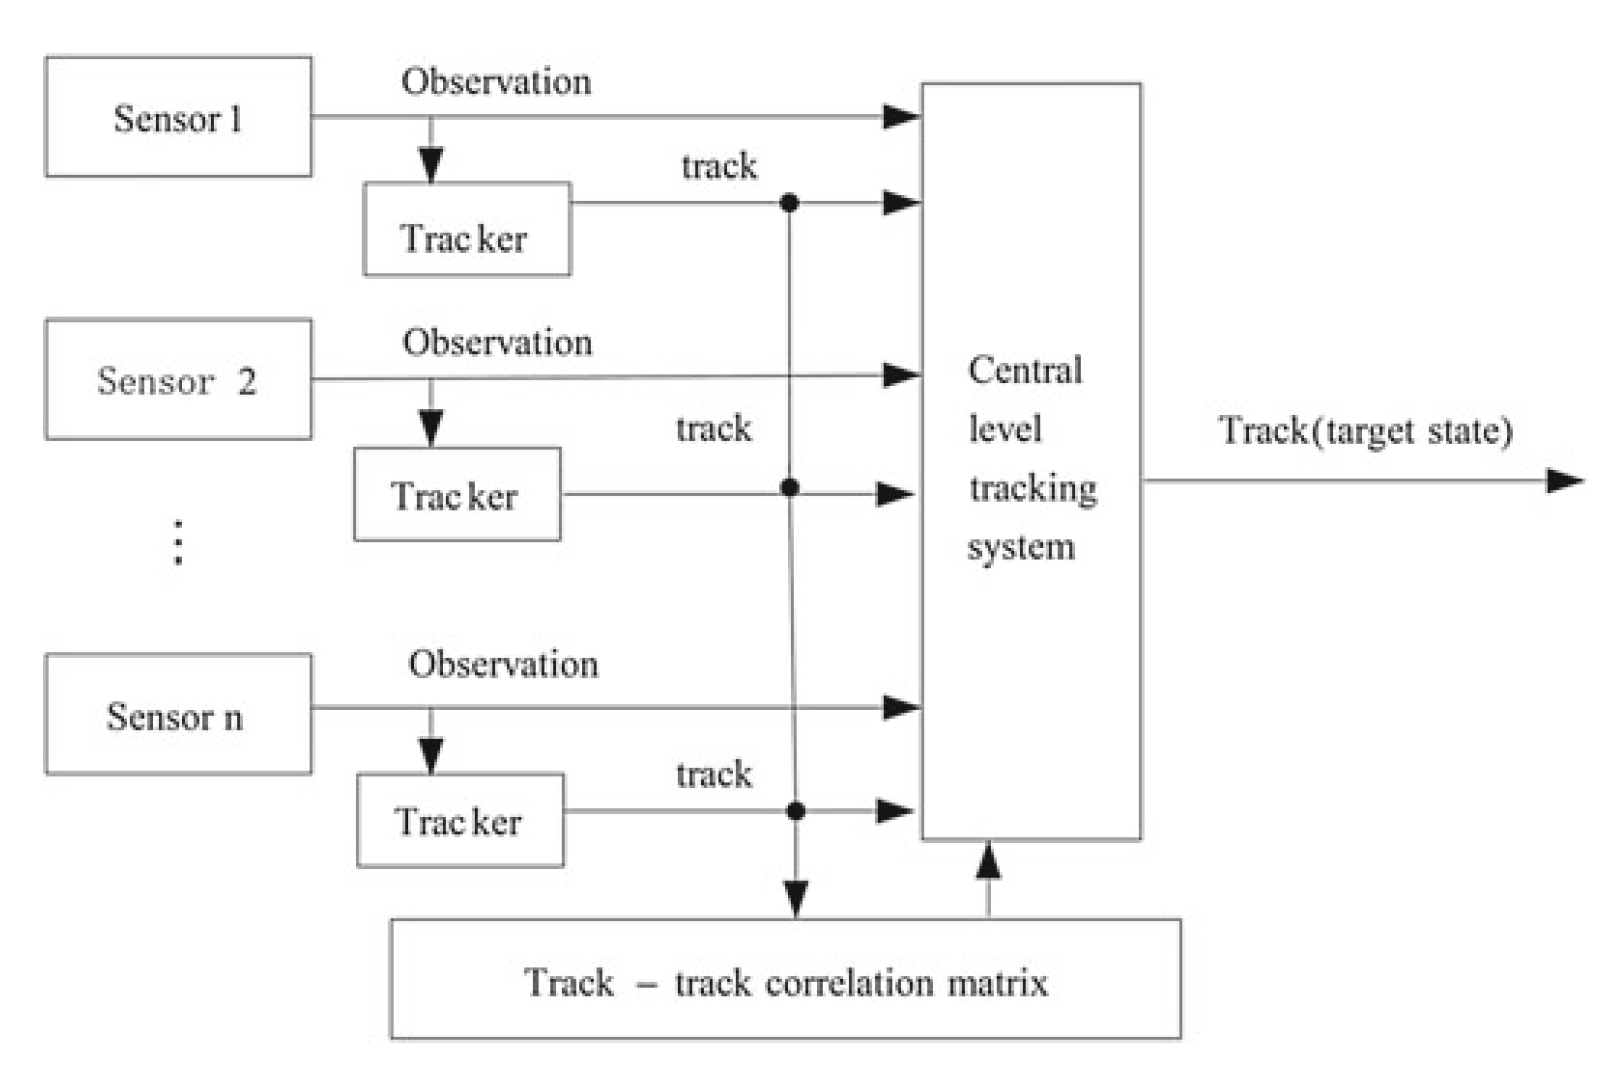
\includegraphics[width=0.9\textwidth]{Images/hybrid.png}
    \caption{Compound Fusion Architecture \cite{yan}}
    \label{hybrid}
\end{figure}

\subsection{Compound Fusion Architecture}
Compound fusion structure is a combination of centralized and distributed fusion framework where the detection report from the sensor modality with tracking information from the local nodes are sent to the central node as shown in Fig. \ref{hybrid}. Such type of structure requires an advanced processing logic because it synthesizes the detection report and tracking information in addition to optimizes combinations. Although it requires complex communication and long processing time, it is used in many applications such as cruise missile control, and radar-based guidance system.

\section{Linear Kalman Filtering}
\label{linearkalmaanfilter}
The Kalman filter (KF) is a Bayesian filter that uses on Gaussian probability density function to estimate the target state. The target state is considered as a random variable. By defining the dynamic model and measurement model of the system, the Kalman filter describes the relationship between target state and measurement. Based on the minimum mean square error estimation criterion, the Kalman filter is an optimal filter. It performs the sequential calculations to predict the target state by using a dynamic model and further update it or make corrections in prediction by using measurements.  

The implementation of a linear Kalman filter for the discrete-time dynamic system is as follows.

\begin{equation}
x_{k}=F_{k-1} x_{k-1}+G_{k-1} u_{k-1}+w_{k-1}
\end{equation}

\begin{equation}
z_{k}=H_{k} x_{k}+v_{k}
\end{equation}

Where, $x_{k}$ is a state vector at time stamp $k$, $F_{k-1}$ is a state transition metric, $G_{k-1}$ is a control gain, $u_{k-1}$ is a control input, $w_{k-1}$ is a process noise at time $k-1$, $z_{k}$ is a measurement vector from sensor at time $k$,  $H_{k}$ is a measurement metric, and $v_{k}$ is a measurement noise.

The measurement noise $v_{k}$ and process noise $w_{k-1}$ are considered as a zero-mean uncorrelated white noise. The measurement co-variance $R_{k}$ and process co-variance $Q_{k}$ are defined as follow. 

\begin{equation}
    Q_{k} = E{w_{i} w_{j}^T} = 
    \left[\begin{array}{ccc}
    q_{xx} & 0 & 0 \\
    0 & q_{yy} & 0 \\
    0 & 0 & q_{zz}
    \end{array}\right] \\
    R_{k} = E{v_{i} v_{j}^T} =
    \left[\begin{array}{ccc}
    r_{xx} & 0 & 0 \\
    0 & r_{yy} & 0 \\
    0 & 0 & r_{zz}
    \end{array}\right]
\end{equation}

The state initialization $x_{0}$ is assumed to be follow the Gaussian distribution with mean $\bar{x_{o}}$ and co-variance $P_{0}$.

\begin{figure}
    \centering
    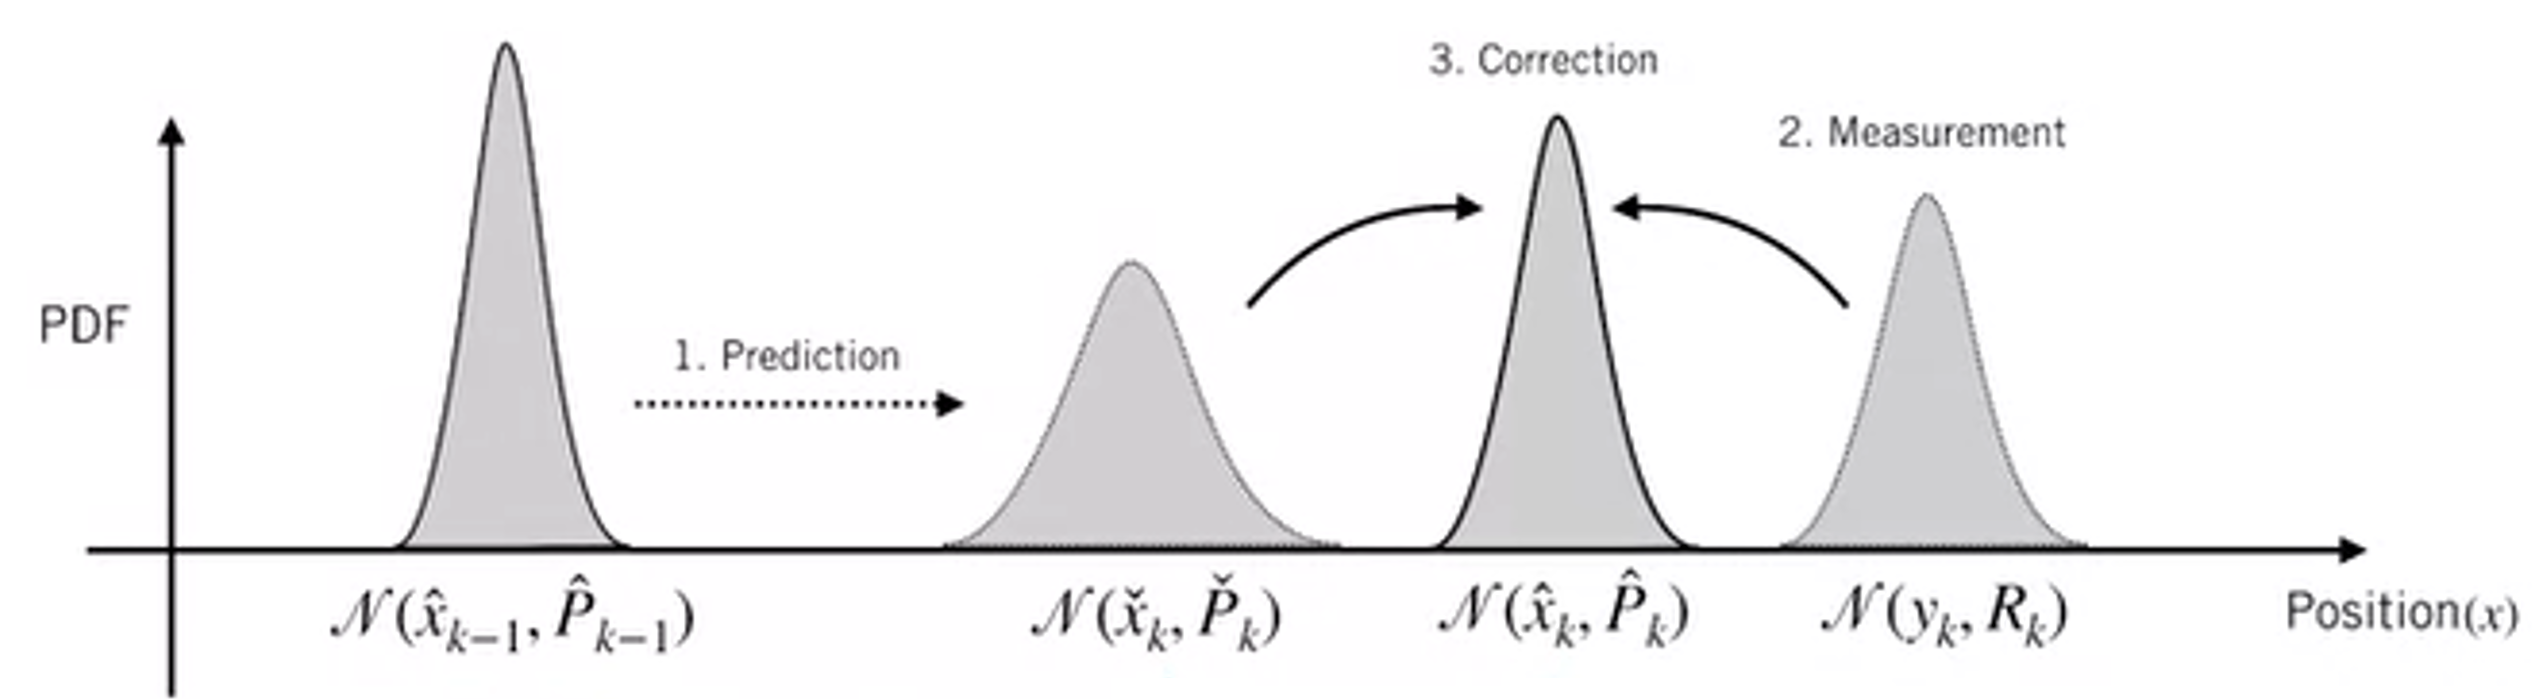
\includegraphics[width=0.9\textwidth]{Images/KF.png}
    \caption{State and Co-variance Propagation in Prediction and Correction Steps \cite{coursera2}}
    \label{KF}
\end{figure}

\textbf{Prediction:}
In the prediction step, the state estimation of previous time stamp $x_{k}$ is substituted in dynamic model to propagate the state forward at discrete time stamp $k+1$ as $x_{k+1|k}$. Similarly, the prediction co-variance is also propagated as $P_{k+1|k}$. 

\begin{equation}
\begin{array}{l}
x_{k+1 / k}=F_{k} x_{k / k}+G_{k / k} u_{k} \\
P_{k+1 / k}=F_{k} P_{k / k} F_{k}^{T}+Q_{k}
\end{array}
\end{equation}

\textbf{Correction:}
In the correction step, estimated states are corrected by using measurements through feedback. It means the discrepancy between predicted measurement $x_{k+1|k}$ and actual measurement $y_{k+1}$ is added to the state estimation after multiplying with feedback gain metric $K_{k+1}$ (Kalman Gain) and the estimation co-variance also corrected as mention in Eq.(\ref{correction}).

\begin{equation}
K_{k+1}=P_{k+1 / k} H_{k+1}^{T}\left(H_{k+1} P_{k+1 / k} H_{k+1}^{T}+R_{k+1}\right)^{-1}
\end{equation}

\begin{equation}
\label{correction}
\begin{array}{l}
x_{k+1 / k+1}=x_{k+1 / k}+K_{k+1}\left(\tilde{z}_{k+1}-H_{k+1} x_{k+1 / k}\right) \\
P_{k+1 / k+1}=\left(1-k_{k+1} H_{k+1}\right) p_{k+1 / k}
\end{array}
\end{equation}

\section{Multi-Sensor Data Fusion}
In multi-sensor data fusion implementation, the sequential update of measurements from more than one sensor can be done in two ways based on sensor synchronization.  

\begin{figure}
    \centering
    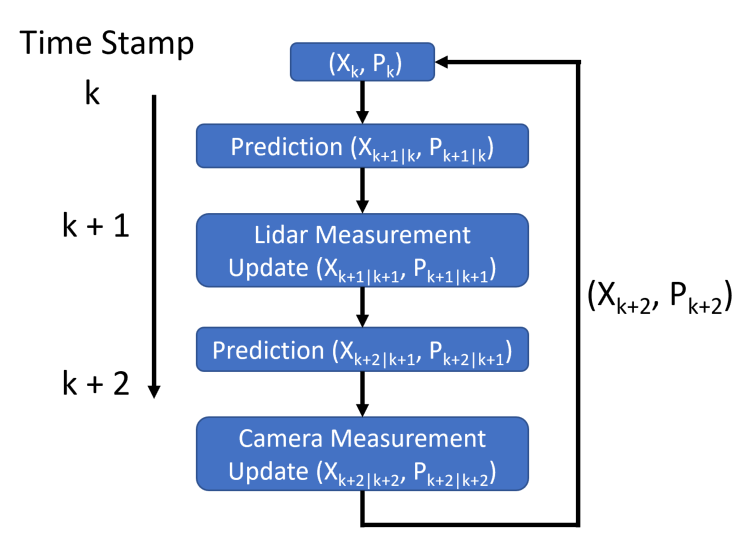
\includegraphics[width=0.9\textwidth]{Images/fusion.png}
    \caption{Flowchart of Multi-sensor Data Fusion for Asynchronous Case}
    \label{fusion}
\end{figure}

\textbf{1: Synchronous Case}
In an asynchronous case, a measurement from each sensor available at each sampling time. In this case, the measurements from all sensors are stacked and simultaneous measurement update is carried out. 

\textbf{2: Asynchronous Case}
In this case, the measurements are available asynchronously at each timestamp. The prediction and update steps are carried out in the order in which the measurements are obtained. A flowchart for camera and LiDAR data fusion is illustrated in Fig. \ref{fusion}.



